\setcounter{section}{0}
\newpage
\begin{center}
  \huge{Codierungstheorie}
\end{center}

\section{Grundbegriffe und einfache Beispiele}
	\subsection{Codierung (Kanalcodierung)}
		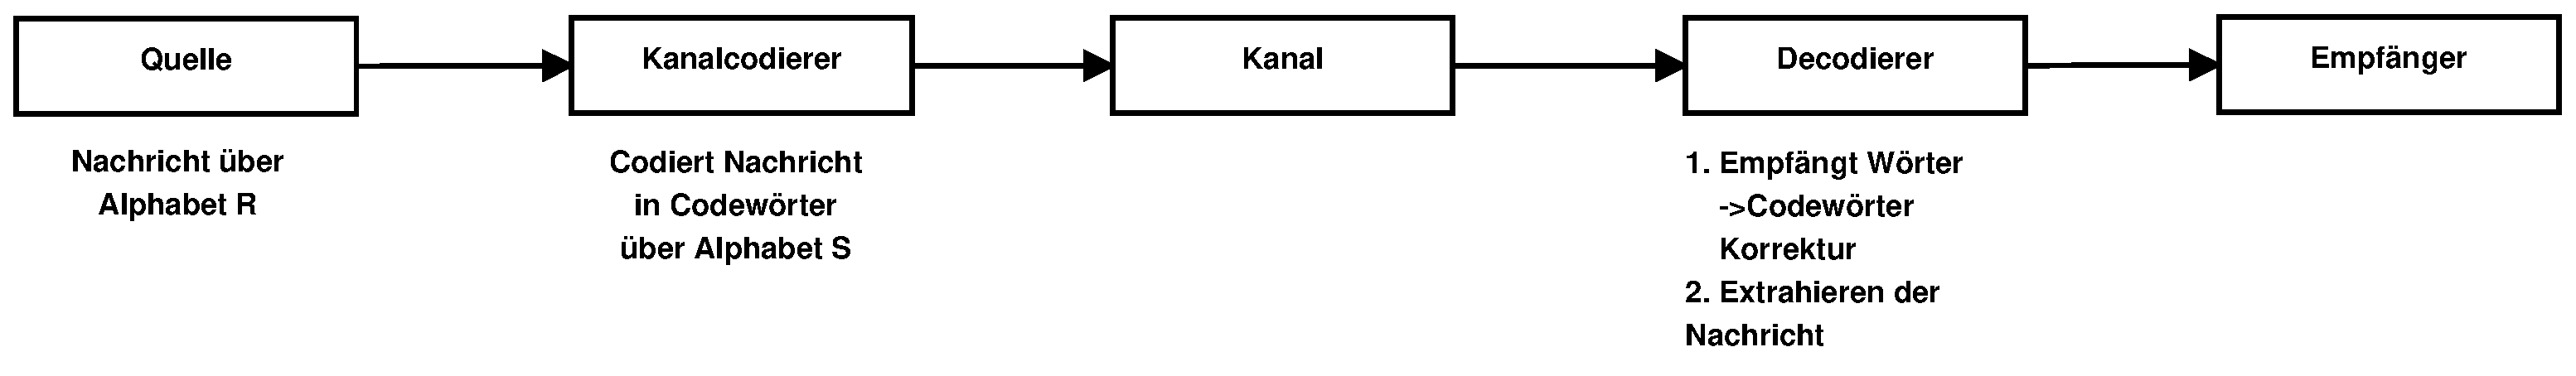
\includegraphics[width=\textwidth]{eps/pic02.eps}
		Die Ziele von Kanalcodierung sind:
		\begin{itemize}
			\item Sicherung von Daten bei Übertragung / Speicherung gegen Störungen, Fehler, etc.
			\item Möglichst viele Fehler erkennen und gegebenfalls korrigieren.
			\item Aufwand für Codierung und Decodierung soll nicht zu hoch sein.
		\end{itemize}
		Grundprinzip: Hinzufügen systematischer Redundanz.\\
		Fehlererkennung: Geringe Redundanz\\
		Fehlerkorrektur: Größere Redundanz, größerer Aufwand
	
	\subsection{Beispiele}
		\begin{enumerate}[a)]
			\item Parity- Check- Code
				$R=\lrc{0,1}$\\
				Nachricht wird in Blöcke von Länge $k$ zerlegt. Füge an jeden Block Bit an, so dass die Anzahl der Einsen im Block der Länge $k+1$ gerade ist (also 1 für ungerade, 0 für gerade).\\
				$k=2$:\\
				$00\rightarrow 000\\
				01\rightarrow 011\\
				10\rightarrow 101\\
				11\rightarrow 110$\\
				1 Fehler wird erkannt (kann nicht korrigiert werden). 2 Fehler können nicht erkannt werden.
			\item Wiederholungscode: Nachricht zerlegt in Blöcke der Länge $k$. Jeder Block wird $m$ mal gesendet. $k=2$, $m=3$\\
				$00\rightarrow 000000\\
				01\rightarrow 010101\\
				10\rightarrow101010\\
				11\rightarrow111111$\\
				1 Fehler lässt sich korrigieren.
			\item Codiere Blöcke der Länge 2 wie folgt:\\
				$00\rightarrow 00000\\
				01\rightarrow 01101\\
				10\rightarrow 10110\\
				11\rightarrow 11011$\\
				1- Fehler- korrigierend:\\
				Decodierung: Such das \gqm{nächste} Codewort zum empfangenen Wort. Je zwei\\Codewörter unterscheiden sich an mindestens 3 Stellen.\\
				2- Fehler- erkennend: Kann jedoch nicht korrigiert werden, da Abstand zu\\
				zwei gültigen Worten 2 ist.
		\end{enumerate}

	\subsection{GTIN- Prüfzifferncode (GTIN-13)}
		\begin{enumerate}[a)]
			\item GTIN=Global Trade Item Number (früher EAN-13)\\
				12- stelliger Code, $R=S=\lrc{0,...,9}$. Erste 12 Ziffern ensprechen
				Information, 13. Ziffer ist die Prüfziffer\\
				$c_1...c_{13}:c_1...c_{12}$\\
				Herstellungsland (in der Regel die ersten drei Ziffern, Deutschland: 400-440)\\
				Hersteller (in der Regel $c_4,...,c_8$ (4-6 Ziffern)\\
				Produkt (in der Regel $c_9,...,c_{12}$ (3-5 Ziffern)\\
				$c_{13}$ wird so gewählt, dass gilt:
				$c_1+3c_2+c_3+3c_4+...+c_{11}+3c_{12}+c_{13}\equiv 0(\mod 10)$\\
				$c_{13}=(-c_1+3c_2-c_3-...-3c_12)\mod 10$\\
				Änderung einer Ziffer wird erkannt. $x\mapsto 3x\mod 10$ ist bijektiv
				($\ggT(3,10)=1$)
			\item Übersetzung der GTIN- 13 in Barcode:\\
				Exkurs, spar ich mir.
		\end{enumerate}

\section{Blockcodes}
	\subsection{Definition}
		$S$ endliche Menge (Alphabet), $n\in\mn$\\
		\textbf{Blockcode} $\mathcal{C}$ der \textbf{(Block-)Länge} $n$ über $S$ ist Teilmenge von $S^n=S\underbrace{\times\dots\times}_{n}S$.\\
		Elemente von $\mathcal{C}$: \textbf{Codewörter}\\
		$S=\lrc{0,1}$: \textbf{binärer Blockcode}\\
		Klar ist $\lrabs{\mathcal{C}}\leq\lrabs{S^n}=\lrabs{S}^n$\\
		Ist $\lrabs{\mathcal{C}}=m$, so lassen sich $m$ Informationssymbole (oder Blöcke) durch je ein Codewort codieren.
	
	\subsection{Definition: Hamming- Abstand}
		$S$ endliches Alphabet, $n\in\mn$\\
		$a=\lrr{s_1,\dots,s_n}, b=\lrr{t_1,\dots,t_n}\in S^n$\\
		$d\lrr{a,b}=\lrabs{\lrc{i:1\leq i\leq n, s_i\neq t_i}}$ \textbf{Hamming-Abstand} von $a$ und $b$\\
		(R.W. Hamming, 1915-1998; C. Shannon)
		
	\subsection{Bemerkung}
		\subExBegin{a)}
			\item $a,b,c\in S^n$. Dann gilt $d\lrr{a,c}\leq d\lrr{a,b}+d\lrr{b,c}$ (Dreiecksungleichung)\\
				$a=\lrr{a_1,\dots,a_n}, b=\lrr{b_1,\dots,b_n}, c=\lrr{c_1,\dots,c_n}$\\
				Es gilt $a_i\neq c_i\Rightarrow a_i\neq b_i$ oder $c_i\neq b_i$
			\item Ist $S$ abelsche Gruppe (bzgl. $+$), so gilt\\
				$\forall a,b,c\in S^n: d\lrr{a,b}=d\lrr{a+c,b+c}$\\
				$\lrr{a_1,\dots,a_n}+\lrr{c_1,\dots,c_n}:=\lrr{a_1+c_1,\dots, a_n+c_n}$
			\item Wird $x\in\mathcal{C}$ gesendet und $y\in S^n$ empfangen und $d\lrr{x,y}=k$, so sind $k$ Fehler aufgetreten.
		\subExEnd
	
	\newpage
	\subsection{Definition}
		\subExBegin{a)}
			\item \textbf{Hamming-Decodierung} für Blockcode $\mathcal{C}\mpo S^n$\\
				Wird $y\in S^n$ empfangen, so wird $y$ als ein $x'\in\mathcal{C}$ decodiert mit\\
				$d\lrr{x',y}=\min\lrc{d\lrr{x,y}:x\in\mathcal{C}}$ (nicht notwendig eindeutig!)\\
				Hamming-Decodierung ist bestmöglich, wenn alle Codewörter mit der gleichen\\Wahrscheinlichkeit $p<\frac{1}{2}$ gestört werden und wenn jedes Codewort gleich wahrscheinlich ist.
			\item $\mathcal{C}$ Blockcode in $S^n$, $\lrabs{\mathcal{C}}>1$\\
				\textbf{Minimalabstand} $d\lrr{\mathcal{C}}$ von $\mathcal{C}$: $d\lrr{\mathcal{C}}=\min\lrr{\lrc{d\lrr{x,y}:x,y\in\mathcal{C}:\ x\neq y}}$
			\item Blockcode $\mathcal{C}$ heißt \textbf{t-Fehler-korrigierend}, falls $d\lrr{\mathcal{C}}\geq 2t+1$, $\mathcal{C}$ heißt \textbf{t-Fehler-erkennend}, falls $d\lrr{\mathcal{C}}\geq t+1$
		\subExEnd
		
	\subsection{Bemerkung}
		\subExBegin{a)}
			\item Ist $d\lrr{\mathcal{C}}\geq 2t+1$, so sind die \gqm{Kugeln} vom Radius $t$ um Codewörter $x\in\mathcal{C}$, $K_t\lrr{x}=\lrc{y\in S^n: d\lrr{x,y}\leq t}$, sind disjunkt.\\
				Angenommen $x\in\mathcal{C}$ wird gesendet, $y\in S^n$ wird empfangen, maximal $t$ Fehler seien aufgetreten $(d\lrr{x,y}\leq t)$. Bei Hamming-Decodierung wird dann $y$ wieder zu $x$ decodiert, denn jedes andere $x'\in\mathcal{C}$ hat Abstand $>t$ von $y$.
				
			\item Ist $d\lrr{\mathcal{C}}\geq t+1$, $x\in\mathcal{C}$ wird gesendet, $y\in S^n$ empfangen, max. $t$ Fehler seien aufgetreten. $d\lrr{x,y}\leq t$. Also ist $y\notin\mathcal{C}$ (falls mindestens ein Fehler aufgtreten ist).
		\subExEnd
		
	\subsection{Beispiele}
		\subExBegin{a)}
			\item Parity-Check-Code\\
				$\mathcal{C}=\lrc{\lrr{c_1,\dots,c_n}:c_i\in\mz^2,\sum c_i\equiv 0\lrr{\mbox{mod }2}}$\\
				$d\lrr{\mathcal{C}}=2$\\
				$\lrr{c_1,\dots,c_{n-2},c_{n-1},c_n}\in\mathcal{C}$\\
				$\lrr{c_1,\dots,c_{n-2},\overline{c_{n-1}},\overline{c_n}}\in\mathcal{C}$\\
				$\Rightarrow\mathcal{C}$ ist $1$-Fehler-erkennend.
			\item $m$-facher-Wiederholungscode: $d\lrr{\mathcal{C}}=m$\\
				$\mathcal{C}=\lrc{\lrr{0,\dots,0},\lrr{1,\dots,1},\lrr{2,\dots,2},\dots}$\\
				$\mathcal{C}$ ist $\floor{\frac{m-1}{2}}$-Fehler-korrigierend.\\
				$d\lrr{\mathcal{C}}\geq 2t+1$ Für alle $x,x'\in \mathcal{C}, x\neq x': K_t\lrr{x}\mand K_t\lrr{x'}=\mvoid$
		\subExEnd
		
	\subsection{Definition: Perfekte Codes}
		Sei $\mathcal{C}$ Blockcode über $S$ der Länge $n$.
		$\mathcal{C}$ heißt \textbf{perfekt}, falls es $t\in\mn_0$ gibt mit \[S^n=\bigcup_{x\in\mathcal{C}}^{\cdot}K_t\lrr{x}\quad\mbox{(disjunkte Vereinigung)}\]
	
	\subsection{Bemerkung}
		Ist $ \mathcal{C} $ perfekt, $ \lrabs{\mathcal{C}}>1 $, $ t $ wie in 8.7, dann ist $ d(\mathcal{C})=2t+1 $.
		
		\textbf{Beweis:} Klar: $ d(\mathcal{C})>t $. Angenommen, $ d(\mathcal{C})\leq $. Wähle $ x,x'\in\mathcal{C} $ mit $ d(x,x')=d(\mathcal{C}) $. Wähle $ y\in S^n $ mit $ d(x,y)=t,\ d'(x',y)\leq t $\\
		Dann; $ x\in K_t(x)\mand K_t(x') $ \lightning.\\
		Also $ d(\mathcal{C})\geq 2t+1 $\\
		Wähle $ x\in\mathcal{C} $. Wähle $ y\in S^n $ mit $ d(x,y)=t+1 $. $ y\notin K_t(x) $. $ \mathcal{C} $ perfekt. $ \exists x'\in\mathcal{C} $ mit $ y\in K_t(x') $. $ d(x,x')\leq d(x,y)+d(y,x') \leq t+1+t=2t+1 $\\
		Also: $ d(\mathcal{C})\geq 2t+1 $
		
	\subsection{Lemma}
		$ \lrabs{S}=q $, $ x_t\in S^n $, $ t\in\mn_0 $. Dann ist
		\[\lrabs{K_t(x)}=\limsum{i=0}{t}\binom{n}{i}(q-1)^i\]
		
		\textbf{Beweis:} $ x\in S^n $. Wie viele Wörter haben Abstand $ i $ von $ x $?\\
		Wähle $ i $ Positionen aus $ \lrc{i,...,n} $ aus: $ \binom{n}{i} $ Möglichkeiten.
		Bei Auswahl dieser Positionen: $ (q-1)^i $ Möglichkeiten, ein Wort auszuwählen, dass sich von $ x $ an diesen $ i' $ Positionen unterscheidet. Also gibt es insgesamt $ \binom{n}{i}(q-1)^i $ Wörter, die den Abstand $ i $ haben. In einer Kugel müssen diese noch aufsummiert werden.
		
	\subsection{Satz}
		Sei $ \mathcal{C} $ ein Code der Länge $ n $ über $ S $, $ \lrabs{\mathcal{C}}>1 $, $ \lrabs{S}=q $. Sei $ t\in\mn_0 $ maximal mit $ d(\mathcal{C})\geq 2t+1 $, d.h. $ t=\lfloor\frac{d(\mathcal{C}) -1}{2}\rfloor $.
		\begin{enumerate}[a)]
			\item  Hamming- Schranke, Kugelpackungsraum $ K_0 $.
			\[\lrabs{\mathcal{C}}\leq\dfrac{q^n}{\limsum{i=0}{t}\binom{n}{i}(q-1)^i}\]
			\item  $ \mathcal{C} $ ist perfekt $ \Leftrightarrow $ \[\lrabs{\mathcal{C}}=\dfrac{q^n}{\limsum{i=0}{t}\binom{n}{i}(q-1)^i}\]
		\end{enumerate}
		
		\textbf{Beweis:}
		\begin{enumerate}[a)]
			\item $ S^n\mpo\bigcup\limits_{x\in\mathcal{C}}^{\cdot} K_t(x)\ \Rightarrow\ q^n=\lrabs{S^n}\geq\lrabs{\bigcup\limits_{x\in\mathcal{C}}^{\cdot}K_t(x)}=\limsum{x\in\mathcal{C}}{}\lrabs{K_t(x)}\ouset{=}{}{\mbox{\scriptsize 8.9}}\mathcal{C}\cdot\limsum{i=0}{t}\binom{n}{i}(q-1)^i $.
			\item  Gleichheit:\\
			$ \leftrightarrow S^n=\bigcup\limits_{x\in C}^{\cdot}K_t(x)\ \Leftrightarrow\ C $ perfekt.
		\end{enumerate}
	
	\subsection{Beispiel}
		Skip
		
	\subsection{Beispiele für perfekte Codes}
		a) - c) trivial perfekte Codes
		\begin{enumerate}[a)]
			\item Einelementige Codes ($ t=n $)
			\item $ \mathcal{C}=S^n\quad (t=0) $
			\item  $ n=2t+1 $, $ \mathcal{C}=\lrc{(0,...,0),(1,...,1)} $ perfekt
			\item $ S=\mz_2=\lrc{0,1} $\\
			$ \mathcal{C}=\{(c_1,...,c_7)\in\mz_2^7:c_1+c_4+c_6+c_7=0,\ c_2+c_4+c_5+c_7=0,\  c_3+c_5+c_6+c_7=0\} $\\
			$ \lrabs{\mathcal{C}}=2^4,\ d(\mathcal{C})=3 $ (nachrechnen)\\
			\textbf{links:} $ \lrabs{\mathcal{C}}=2^4 $\\
			\textbf{rechts:} $ \frac{2^7}{1+7}=2^4 $\\
			\textbf{Hamming- Code}
		\end{enumerate}
		
\section{Lineare Codes}
	\subsection{Definition}
		$ K $ endlicher Körper, $ n\in\mn $.\\
		Ein \textbf{linearer Code} $ \mathcal{C} $ ist ein Unterraum des Vektorraums $ K^n $ (d.h. $\alpha=k $).\\
		Ist $ \dim(\mathcal{C})=k\ (k\leq n) $, so heißt $ \mathcal{C} $ ein $ [n,k] $- Code.\\
		Ist $ \lrabs{K}=q $, $ \dim(\mathcal{C})=k $, dann $ \lrabs{\mathcal{C}}=q^k $.\\
		$ \mathcal{C} $ hat Basis $ w_1,...,w_k $, $ \mathcal{C}=\lrc{a_1w_1+...+a_kw_k:\ a_i\in K} $
	
	\subsection{Bemerkung}
		$ \mz_p=\lrc{0,...,p-1} $ ist Körper bezüglich Addition und Multiplikation $ \mod p $, falls $ p $ eine Primzahl ist.\\
		Körper von Ordnung $ p^m $: Irreduzibles Polynom $ g $ vom Grad $ m $ über $ \mz_p $.\\
		$ K=\lrc{f\in\mz_p[x]:\grad(f)<m} $, $ \lrabs{K}=p^m $\\
		Addition und Multiplikation $ \mod g $.\\
		(Bis auf Isomorphie) gibt es keine anderen endlichen Körper.
		
	\subsection{Beispiel}
		\subExBegin{a)}
		\item $ n $- facher Wiederholungscode über $ \mz_p $.\\
		$ \mathcal{C}=\lrc{(0,...,0),(1,...,1),...,(p-1,...,p-1)}=\lrg{(1,...,1)} $ $ [n,1] $- Code über $ \mz_p $.\\
		$ d(\mathcal{C})=n $
		\item Hamming- Code (8.12 d)) ist \textbf{linearer} $ [7,4] $- Code über $ \mz_2 $, $ d(\mathcal{C})=3 $ (als Lösungsraum eines homogenen, linearen LGS über $ \mz_2 $).
		\item $ n\geq 2 $. $ \mathcal{C}=\lrc{(c_1,...,c_n):\ \limsum{i=1}{n}c_i=0}\mpo K^n $ linearer $ [n,n-1] $- Code.\\
		$ K=\mz_2 $: Parity- Check- Code
		\subExEnd
		
	\subsection{Definition: (Minimal-) Gewicht}
		$ K $ endlicher Körper.
		\begin{enumerate}[a)]
			\item $ x= (x_1,...,x_n)\in K^n$. $ wt(x)=d(x,0)=\lrabs{\lrc{i:\ x_i\neq 0}} $ Gewicht von $ x $.
			\item Ist $ \lrc{0}\neq\mathcal{C}\mpo K^n $, so heißt $ wt(\mathcal{C})=\min\lrc{wt(x):\ 0\neq x\in\mathcal{C}} $\\
			Minimalgewicht von $ \mathcal{C} $.
		\end{enumerate}
		
	\subsection{Satz}
		Ist $ \lrc{0}\neq\mathcal{C} $ ein linearer Code, so ist $ d(\mathcal{C})=wt(\mathcal{C}) $.
		
		\textbf{Beweis:} $ \mathcal{C} $ linear, $ x,x'\in\mathcal{C}\ \Rightarrow\ x-x'\in\mathcal{C} $.\\
		$ d(\mathcal{C})=\min\lrc{d(x,x'):\ x,x'\in\mathcal{C},\ x\neq x'} $\\
		$ =\min\lrc{d(\underbrace{x-x'}_{\in\mathcal{C}},0):\ x,x'\in\mathcal{C},\ x\neq x'} $\\
		$ =\min\lrc{d(y,0):\  \neq y\in\mathcal{C}}=wt(\mathcal{C}) $.
		
	\subsection{Definition: Generatormatrix}
		$\mathcal{C}\lra{n,k}$-Code über $K$.\\
		Sei $g_1=\lrr{g_{11},\dots,g_{1n}},\dots,g_k=\lrr{g_{k1},\dots,g_{kn}}$ Basis von $\mathcal{C}$\\
		$G=\lrv{g_1\\\vdots\\g_k}=\lrv{g_{11}\dots g_{1n}\\\vdots\\g_{k1}\dots g_{kn}},\; k\times n$-Matrix, \textbf{Erzeugermatrix} (\textbf{Generatormatrix}) von $\mathcal{C}$

	\subsection{Satz}
		$G$ Erzeugermatrix von $\lra{n,k}$-Code $\mathcal{C}$. Dann gilt $\mathcal{C}=\lrc{uG\mid u\in K^k}$.

		\textbf{Beweis}

		$u=\lrr{u_1,\dots,u_k}, uG=\lrr{u_1,\dots,u_k}\lrv{g_1\\\vdots\\g_k}=u_1g_1+\dots+u_kg_k\in\mathcal{C}$\\
		Auf diese Weise erhält man alle \textbf{Elemente} von $\mathcal{C}$

	\subsection{Bemerkung}
		\begin{enumerate}[a)]
			\item Abbildung $\begin{cases} K^k\rightarrow\mathcal{C}\mpo K^n\\u\mapsto u\cdot G\end{cases}$ ist bijektiv.\\
				Es ergibt sich die Codierungsmöglichkeit:\\
				Infowörter der Länge $k\rightarrow$ Codewörter der Länge $n$\\
				(Lineare Algebra: Es existiert Matrix $\ouset{G}{\sim}{}, n\times k, G\cdot\ouset{G}{\sim}{}=E_k$\\
				$c\in\mathcal{C}, c=uG$, Bilde $c\ouset{G}{\sim}{}=uG\ouset{G}{\sim}{}=uE_k=u$)
			\item Elementare Zeilenumformungen bilden aus Erzeugermatrix $G$ von $\mathcal{C}$ wieder eine \\Erzeugermatrix von $\mathcal{C}$.
		\end{enumerate}

	\subsection{Beispiel}
		Hamming $\lra{7,4}$-Code über $\mz_2=\lrc{0,1}$\\
		$\mathcal{C}=\lrc{c_1,\dots,c_7\in\mz_2^7:c_1+c_4+c_6+c_7=0, c_2+c_4+c_5+c_7=0, c_3+c_5+c_6+c_7=0}$\\
		$c_4,c_5,c_6,c_7$ frei wählbar $\rightarrow c_1,c_2,c_3$ sind dann bestimmt.\\
		Basis von $\mathcal{C}$: $\lrv{1&1&1&0&0&0&1},\lrv{1&0&1&0&0&1&0},\lrv{0&1&1&0&1&0&0},\lrv{1&1&0&1&0&0&0}$\\
		Erzeugermatrix $G=\lrv{1110001\\1010010\\0110100\\1101000}\ouset{\Rightarrow}{\smt{elem.}}{\smt{Umf.}}\lrv{1110001\\0100011\\0110100\\0011001}\ouset{\Rightarrow}{\smt{elem.}}{\smt{Umf.}} G'=\lrv{1000101\\0100011\\0010111\\0001110}$ Erzeugermatrix in \textbf{Standardform} von $\mathcal{C}$.(Muss nicht existieren)\\
		Codierung mit $G'$: $\lrv{u_1,u_2,u_3,u_4}G'=\lrv{u_1,u_2,u_3,u_4,u_1+u_3+u_4,u_2+u_3+u_4,u_1+u_2+u_3}\in\mathcal{C}$

	\subsection{Satz und Definition}
		$\mathcal{C}$ sei ein $\lra{n,k}$-Code über $K$. Dann existiert $\lrr{n-k}\times n$-Matrix $H$ so dass gilt:\\
		$y\in K^n: y\in\mathcal{C}\Leftrightarrow Hy^t=0\in K^{n-k}$\\
		$H$ heißt \textbf{Kontrollmatrix} von $\mathcal{C}$\\
		Es ist $\mbox{rg}\lrr{H}=n-k$\\
		(Dann gilt auch $H\cdot G^t=0$, also genau die $\lrr{n-k}\times k$-Nullmatrix, falls $G$ Erzeugermatrix von $\mathcal{C}$)
		
		\newpage
		\textbf{Beweis}\\
		Sei $g_1,\dots,g_k$ Basis von $\mathcal{C}$, $G=\lrv{g_1\\\vdots\\g_k},g_i=\lrr{g_{i1},\dots,g_{in}}$
		LGS:\\
		$x_1g_{11}+\dots+x_ng_{1n}=0\\
		\dots\\
		x_1g_{k1}+\dots+x_ng_{kn}=0$\\
		Das heißt $G\cdot\lrv{x_1\\\vdots\\x_n}=0$ bzw. $\lrr{x_1,\dots,x_n}\cdot G^t=0$\\
		$\mbox{rg}\lrr{G}=k$ Dimension des Lösungsraums ist $n-k$\\
		$h_1,\dots,h_{n-k}$ ist Basis des Lösungsraums,\\
		$Hg_i^t=\lrv{h_1g_i^t\\\vdots\\h_ng_i^t}=0,i=1,\dots,k\Rightarrow Hy^t=0\forall y\in\mathcal{C}$\\
		LGS ($Hy^t$), Koeffizientenmatrix hat Rang $n-k$ Lösungsraum $\mathcal{C}$ hat $\dim\lrr{k}$
		
	\subsection{Bemerkung}
		\begin{enumerate}[a)]
			\item Kontrollmatrix kann zur Fehlererkennung verwendet werden
			\item Beweis von 9.10: Erzeugermatrix $\rightarrow$ Kontrollmatrix umgekehrt analog
		\end{enumerate}

	\subsection{Beispiele}
		\begin{enumerate}[a)]
			\item Parity-Check-Code $\mathcal{C}=\lrc{\lrr{c_1,\dots,c_n}:\sum c_i=0}$\\
				$\lra{n,n-1}$-Code $G$ ist $n\times n$-Einheitsmatrix mit einer zusätzlichen Spalte voller Einsen.
			\item $\lra{7,4}$-Hamming-Code: $H=\lrv{1001011\\0101101\\0010111}$ Kontrollmatrix
			\item $\mathcal{C}$ Code mit Erzeugermatrix $\lrv{1001\\0111}$ $\lra{4,2}$-Code über $\mz_2$\\
				Kontrollmatrix:\\
				$x_1+x_4=0\\
				x_2+x_3+x_4=0$\\
				Basis des Lösungsraums $Hx^t=0$: $\begin{cases}\lrr{1101}\\\lrr{0110}\end{cases}$\\
				Also $H=\lrv{1101\\0110}$ ist Kontrollmatrix von $\mathcal{C}$
		\end{enumerate}

	\subsection{Satz}
		$\mathcal{C}\neq\lrc{0}, K^n$ ein $\lra{n,k}$-Code über $K$ mit Kontrollmatrix $H$. Dann gilt:\\
		$d\lrr{\mathcal{C}}=\mbox{wt}\lrr{\mathcal{C}}=\min\lrc{r\in\mn:\mbox{ es gibt in H r linear abhängige Spalten}}$\\
		$=\max\lrc{r\in\mn:\mbox{ je r-1 Spalten von H sind lin. unabhängig}}$

		\textbf{Beweis}

		Seien $s_1,\dots,s_n$ Spalten von $H$, $s_i\in K^{n-k}$, $\mathcal{C}\neq\lrc{0}, k\geq 1$\\
		$n-k\leq n-1$ Also $s_1,\dots,s_n$ sind linear abhängig\\
		Sei $w\in\mn$ minimal mit, sodass es $w$ linear abhängige Spalten gibt $s_{i_1},\dots,s_{i_w}$\\
		Dann existieren $c_j\in K, j=1,\dots,n$, mit $\ouset{\limsum{j=1}{n}c_j\cdot s_j=0}{}{\smt{(*)}}, c_j\neq 0$ genau für $j=i_1,\dots,i_w$\\
		Dann auch $\limsum{j=1}{n}c_js_j^t=0$\\
		$c=\lrr{c_1,\dots,c_n}\quad \lrr{c_1,\dots,c_n}H^t=\lrr{c_1,\dots,c_n}\lrv{s_1^t\\\vdots\\s_n^t}=0$\\
		$Hc^t=0\Rightarrow c\in\mathcal{C}$. $\mbox{wt}\lrr{c}=w$\\
		$\mbox{wt}\lrr{\mathcal{C}}\leq\mbox{wt}\lrr{c}=w$\\
		Angenommen es existiert $0\neq\overline{c}\in\mathcal{C}, \overline{w}=\mbox{wt}\lrr{\overline{c}}<w$ Dann folgt aus $\overline{c}H^t=0$. Dann folgt wie in (*), dass $\overline{w}$ Spalten von $H$ sind linear abhängig \lightning

	\subsection{Beispiel}
		$\lra{7,4}$-Hamming-Code über $\mz_2$\\
		Kontrollmatrix: $\lrv{1001011\\0101101\\0010111}$\\
		Je zwei Spalten sind linear unabhängig, aber 1.,2.,4. Spalte sind linear abhängig\\
		$\ouset{\Rightarrow}{}{\smt{9.13}} d\lrr{\mathcal{C}}=3$

	\subsection{Satz - Singleton-Schranke}
		$\mathcal{C}$ linearer $\lra{n,k}$-Code mit $d\lrr{\mathcal{C}}=d$, so ist\\
		$d\leq n-k+1$ (d.h. $k\leq n-d+1$)

		\textbf{Beweis}\\
		$\ouset{\Rightarrow}{}{\smt{9.13}} d\leq\mbox{rg}\lrr{H}+1=n-k+1, H$ Kontrollmatrix von $\mathcal{C}$
	
	\subsection{Nebenklassen von Unterräumen}
		$ \mathcal{C} $ Unterraum von $ V=K^n $. Für jedes $ v\in V $ heißt $ v+\mathcal{C}:=\lrc{v+x|x\in \mathcal{C}} $ die \textbf{Nebenklasse} von $\mathcal{C}$ zu $ v $ ($ v\in c+ \mathcal{C} $, da $ v=v+0 $).
		\begin{enumerate}[a)]
			\item $ v_1,v_2\in V $. Dann gilt: $ v_1+ \mathcal{C}=v_2+\mathcal{C} $ oder $ (v_1+\mathcal{C})\mand(v_2+\mathcal{C})=\emptyset $
			\item $ v_1+\mathcal{C}=v_2+\mathcal{C} $ $ \Leftrightarrow $ $ v_1-v_2\in \mathcal{C} $ $ \Leftrightarrow $ $ v_1\in v_2+ \mathcal{C} $.\\
			$ v+\mathcal{C}=\mathcal{C}=\sigma+\mathcal{C} $ $ \Leftrightarrow $ $ v\in \mathcal{C} $
			\item Wähle aus jeder Nebenklasse einen Vektor $ v_i $. Dann gilt $ V=\overset{\cdot}{\bigcup}(v_i+\mathcal{C}) $
			\item  $ V $ VR über endlichem Körper $ K $. Dann $ \lrabs{\mathcal{C}}=\lrabs{v+\mathcal{C}} $ für alle $ v\in V $.
			\item Ist $ \dim(\mathcal{C})=k $, so ist $ \lrabs{\mathcal{C}}=q^k $. $ \lrabs{V}=q^n $, $ \lrabs{v_i+\mathcal{C}}=q^k $. $ \mathcal{C} $ hat genau $ q^{n-k} $ verschiedene Nebenklassen.
		\end{enumerate}

	\subsection{Syndrom- Decodierung von linearer Codes}
		$ \mathcal{C}[n,k] $- Code, $ H $ Kontrollmatrix, $ (n-k)\times n $. $ y\in K^n $.\\
		$ Hy^t\in K^{n-k} $ heißt \textbf{Syndrom} von $ y $.
		\begin{enumerate}[a)]
			\item Ist $ y\in \mathcal{C} $ $ \Leftrightarrow $ $ Hy^t=0 $
			\item $ y_1,y_2\in K^n $. $ y_1,y_2 $ liegen in derselben Nebenklasse von $ \mathcal{C} $ (d.h. $ y_1+\mathcal{C}=y_2+\mathcal{C} $) $ \Leftrightarrow $ $ Hy_1^t=Hy_2^t $\\
			$ [x_1+\mathcal{C}=y_2+\mathcal{C}\Leftrightarrow y_1-y_2\in \mathcal{C}\Leftrightarrow H(y_1,y_2)^t=0\Leftrightarrow Hy_1^t-Hy_2^t=0] $\\
			Angenommen, $ x\in \mathcal{C} $ wurde gesendet, $ y=x+f $ wurde empfangen ($ f $ Fehlervektor), so haben $ y $ und $f$ das gleiche Syndrom.
			
			\textbf{Hamming- Decodierung:} Bestimme in jeder Nebenklasse von $ \mathcal{C} $ einen Vektor kleinsten Gewichtes (muss nicht eindeutig sein). Dies sei der \textbf{Nebenklassenführer}.\\
			$ y\in K^n $, $ Hy^t\ \rightarrow $ Nebenklasse $ y+\mathcal{C} $. Wähle Nebenklassenführer $ e $. Decodiere $ y\rightarrow y-e\in \mathcal{C} $.\\
			Syndrome sind alle Vektoren des $ K^{n-k} $, z.B. $ K=\mz_2 $. Ordne den Nebenklassenführern entsprechend der lexikographischen geordneten Syndrome.\\
			Speichern braucht man nur den Nebenklassenführer.
			
			\textbf{Beispiel:} $ [50,70] $- Code über $ \mz_2 $.\\
			$ \mathcal{C} $ hat $ 2^{50} $ Codewörter mit je $ 70 $ Bit.\\
			$ \mathcal{C} $ hat $ 2^{20} $ Nebenklassen, Nebenklassenführer mit je $ 70 $ Bit $ \rightarrow\approx 8,75 $ MB.
		\end{enumerate}

\section{Beispiele guter Codes}
	\subsection{Hamming- Codes}
		$ K $ endlicher Körper, $ \lrabs{K}=q $, $ q $ Primzahlpotenz. Wähle $ l\in\mn $, konstruiere $ [n,k] $- Code $ \mathcal{C} $ mit $ n=\frac{q^l-1}{q-1} $, $ k=n-l $, $ l\geq 2 $, $d(\mathcal{C})=3$, perfekt.
		
		\textbf{Konstuktion:} $ |K^l\mnot\lrc{0}|=q^l-1 $. Jeder eindimensionale Unterraum enthält $ q-1 $ Vektoren $ \neq 0 $.\\
		Es gibt $ \frac{q^l-1}{q-1} $ viele eindimensionale Unterräume in $ K^l $. Wähle aus jedem der eindimensionalen Unterräume einen Vektor $ \neq 0 $, schreibe ihn als Spaltenvektor der Länge $ l $ in eine Matrix ($ l\times n $- Matrix $ H $, Kontrollmatrix). $ \dim(\mathcal{C})=n-l $.\\
		Minimalanzahl linear abhängiger Spalten in $ H $. Je zwei Spalten sind linear unabhängig. In $ H $ gibt es 3 linear abhängige Spalten:\\
		$ \lrv{a\\0\\0\\\vdots\\0},\lrv{0\\b\\0\\\vdots\\0},\lrv{c\\c\\0\\\vdots\\0} $ linear abhängig.\\
		9.13: $ d(\mathcal{C})=3 $\\
		$ \lrabs{\mathcal{C}}=\frac{q^n}{\limsum{i=0}{1}\binom{n}{i}(q-1)^i} $\\
		$ q^{n-l}=1+n(q-1)=1+\frac{q^l-1}{q-1}(q-1)=q^l $
		
		$d\lrr{\mathcal{C}}\leq n-k+1$ Singleton (Im Fall von $=$ MDS)
	
	\subsection{Beispiel}
		\subExBegin{a)}
			\item $ q=2 $, $ l=3 $, $ n=\frac{2^3-1}{2-1}=7 $\\
				$ H=\lrv{1&0&0&1&0&1&1\\0&1&0&1&1&0&1\\0&0&1&0&1&1&1} $ 8,12 d)
			\item $ q=3 $, $l=3$, $n=\frac{3^3-1}{3-1}=13$ über $ \mz_3 $\\
				$ \lrv{1&0&0&1&1&0&0&1&1&1&1&1&2\\0&1&0&1&2&1&1&0&0&1&1&2&1\\0&0&1&0&0&1&2&1&2&1&2&1&1} $ Kontrollmatrix. $ \dim(\mathcal{C})=10 $, $ \lrabs{\mathcal{C}}=3^{30}=59.049 $
			\item  $ [7,4] $- Hamming- Code aus a)\\
				$ y=(1110110)\in \mathcal{C} $\\
				$ Hy^t=\lrv{0\\0\\1}\neq\lrv{0\\0\\0} $, $ y\in \mathcal{C} $\\
				Es gibt genau ein $ x\in \mathcal{C} $ mit $ d(x,y)=1 $ ($ \mathcal{C} $ perfekt)\\
				$ x $ unterscheidet sich von $ y $ and einer Stelle $ i $.\\
				$ Hy^t=H(x^t+(0,...,0,1,0,...,0))=H(0,...,0,1,0,...,0)=\lrv{h_{1i}\\h_{2i}\\h_{3i}} $\\
				An welcher Stelle von $ H $ steht $ \lrv{0\\0\\1} $? 3. Stelle: Ändere $ y $ an 3. Stelle: $ y\rightarrow x=\underbrace{(1100110)}_{\in \mathcal{C}} $
		\subExEnd
	
	\subsection{Reed-Solomon-Codes}
		\subExBegin{a)}
			\item $K$ Körper, $\lrabs{K}=q$. Wähle $k,n$ mit $1\leq k\leq n\leq q$\\
				$K\lra{x}_k=\lrc{f\in K\lra{x}: \grad\lrr{f}<k}\quad K$-Vektorraum der Dimension $k$\\
				Basis: $1,x,\dots,x^{k-1}$\\
				Wähle $M=\lrr{a_1,\dots,a_n}, q_i\in K, a_i\neq a_j$ für $i\neq j$\\
				Setze $\mathcal{C}=\mathcal{C}_M=\lrc{\lrr{f(a_1),\dots,f(a_n)}:f\in K\lra{x}_k}\mpo K^n$\\
				\textbf{Reed-Solomon-Code} oder Auswertungscode
			
				Klar: $\mathcal{C}$ ist linearer Code.
			
				\subExBegin{(1)}
					\item $\dim\lrr{\mathcal{C}}=k:$\\
						$\alpha:\begin{cases}K\lra{x}_k\rightarrow\mathcal{C}\\f\mapsto\lrr{f(a_1),\dots,f(a_n)}\end{cases}\quad K$-lineare Abbildung (surjektiv)\\
						$\alpha$ ist injektiv: Zeige $\mbox{kern}\lrr{\alpha}=\lrc{\sigma}$\\
						$f\in\mbox{kern}\lrr{\alpha}$, das heißt $f\lrr{a_1}=\dots=f\lrr{a_n}=0$\\
						$f$ hat mindestens $n$ verschiedene Nullstellen in $K$\\
						$\grad\lrr{f}<k\leq n\Rightarrow f=0$\\
						$\dim\lrr{\mathcal{C}}=\dim\lrr{K\lra{x}_k}=k$
					\item Nach (1) ist $\alpha\lrr{1},\alpha\lrr{x},\dots,\alpha\lrr{x^{k-1}}$ Basis von $\mathcal{C}$\\
						Liefert Erzeugermatrix von $\mathcal{C}$\\
						$G=\lrv{1&\dots&1\\a_1&\dots&a_n\\a_1^2&\dots&a_n^2\\a_1^{k-1}&\dots&a_n^{k-1}}$
					\item $d\lrr{\mathcal{C}}=n-k+1$ hat höchstens $k-1$ Nullstellen. Das heißt jedes Codewort $\lrr{\neq 0}$ hat mindestens Gewicht $n-\lrr{k-1}=n-k+1$, also $\mbox{wt}\lrr{\mathcal{C}}\geq n-k+1$\\
						Setze $f=\lrr{x-a_1}\cdot\dots\cdot\lrr{x-a_{k-1}}\in K\lra{x}_k$\\
						$\mathcal{C}\supseteq\lrr{f(a_1),\dots,f(a_n)}=(\underbrace{0,\dots,0}_{k-1},\underbrace{*,\dots,*}_{\neq 0}$) Gewicht $n-k+1$
					\item Reed-Solomon-Codes sind MDS-Codes
				\subExEnd
			\item Spezielle Reed-Solomon-Codes\\
				$n=q-1, a_i=a^{i-1}\quad i=1,\dots, q-1=n$, wobei $a$ erzeugendes Element der multiplikativen Gruppe $K^*=K\mnot\lrc{0}=\lrc{a^0=1,a^1=a,\dots,a^{1-2}}$\\
				$G=\lrv{1&1&\dots&1\\1&a&a^2&\dots&a^{q-2}\\1&a^2&a^4&\dots&a^{2\lrr{q-2}}\\1&a^{k-1}&a^{2\lrr{k-1}}&\dots&a^{\lrr{k-1}\lrr{q-2}}}$\\
				$d=d\lrr{\mathcal{C}}=n-k+1\quad RS_q\lrr{d}=q-k$\\
				$a\cdot\lrr{1,a,a^2,\dots, a^{q-2}}=\lrr{a,a^2,a^3,\dots,a^{q-2},1}\in\mathcal{C}$
			
				In $RS_q(d)$ ist ein zyklischer Shift jedes Codeworts wieder ein Codewort: \textbf{zyklischer Code}
			
				Anwendung: Codierung von Audio-CD's. Häufigster Fehler: Auslöschungen
		\subExEnd
	
	\subsection{Lemma}
		Linearer Code $\mathcal{C}$, $d\lrr{\mathcal{C}}=d, c\in\mathcal{C}$. Bei Übertragung entstehen bis zu $d-1$ Auslöschungen, aber keine weiteren Fehler, dann lässt sich das empfangene Wort korrekt decodieren.
	
		Suche Codewort, das an den nicht ausgelöschten stellen mit $y$ übereinstimmt.\\
		Gäbe es zwei $c,C'$, so $d\lrr{c,c'}\leq d-1\Rightarrow c=c'$
	
	\subsection{Cross-Interlearing}
		$\mathcal{C}_1, \mathcal{C}_2\;\; \lra{k_i,n_i}$-Codes mir $i=1,2$ Erzeugermatrix in Standardform $G_i=\lrr{E_{k_i}\mid T_i}, i=1,2$\\
		Gegeben seien $k_1$ Informationswörter der Länge $k_2$\\
		$i_1=\lrr{c_{11},\dots,c_{k_21}},\dots,i_{k_1}=\lrr{c_{1k_1},\dots,c_{k_2,k_1}}$\\
		Codiere mit $\mathcal{C}_2$ (\textbf{äußerer Code}), $i_1,\dots,i_{k_1}\rightarrow c_j=(i_j\underbrace{*\dots*}_{n_2-k_2})$\\
		Schreibe $c_1,\dots,c_{k_1}$ als Spalten in Matrix
	
		$n_2\left\lbrace\begin{array}{cccccccc}
			\multicolumn{8}{c}{\longleftarrow n_1 \longrightarrow}\\
			i_1&i_2&\dots&i_{k_1}&*&\dots&*&\in\mathcal{C}_1\\
			*&*&\dots&*&*&\dots&*&\in\mathcal{C}_1\\
			\vdots&\vdots&\vdots&\vdots&\vdots&\vdots&\vdots&\vdots\\
			*&*&\dots&*&*&\dots&*&\in\mathcal{C}_1\\
			\in\mathcal{C}_2&\in\mathcal{C}_2&\dots&\in\mathcal{C}_2&\in\mathcal{C}_2&\in\mathcal{C}_2&\in\mathcal{C}_2&
		\end{array}\right.$
	
		Codiere Zeilen mit \textbf{innerem Code} $\mathcal{C}_1$.\\
		Lese Matrix zeilenweise aus liefert Wort der Länge $n_1\cdot n_2$ mit $k_1\cdot k_2$ Infosymbolen.\\
		Angenommen in $w$ tritt ein Burst-Fehler der Länge $\leq\lrr{d_2-1}\cdot n_1$ auf.
	
		In einer Spalte der Matrix sind maximal $d_2-1$ Einträge betroffen $\mathcal{C}_2$ kann korrigieren.
	
		Audio-CD's: Ausgangscode $RM_{2^8}(5)$ also $\lra{255,251}$-Code\\
		Verkürzung: $\mathcal{C}_1\;\;\lra{32,28}$-Code $d\lrr{\mathcal{C}_1}=5$ und $\mathcal{C}_2\;\;\lra{28,24}$-Code $d\lrr{\mathcal{C}_2}=5$\\
		Bursts der Länge $512$ über $\mathbb{F}_{2^8}$ können korrigiert werden.\\
		Interlering $+$ Interpolarisation $\rightarrow$ Bursts der Länge $\sim 7,5\mbox{ mm}$